\section{Results}
\label{sec:results}

This section reports objective wrap-repair scores under locked $R_{\mathrm{blend}}$
(Sections~\ref{sec:v10-freeze}--\ref{sec:n2n-vs-ours-boards}).
Higher is better. Unless noted, multi-seed cells are mean$\pm$std.
Appendix~\ref{app:supplement} holds the matched outer-loop bake-off, ablations, HP probes, and transfer latency.
Limitations are collected in Section~\ref{sec:limitations}.
The evaluation protocol is stated in Section~\ref{sec:experiments}.

\paragraph{How to read the main numbers.}
\begin{enumerate}
  \item \textbf{Holdout vs Noise2Noise and Dual Cosine} (Table~\ref{tab:n2n-vs-ours}):
    short-FitCell hybrid is close to, but below, Noise2Noise, and far above Dual Cosine.
  \item \textbf{Which outer loop to keep} (Table~\ref{tab:meta-approaches}):
    hybrid has the top descriptive mean in a matched $5$k bake-off ($n{=}3$ search seeds; vs runner-up mean $\Delta{=}{+}0.0114$, bootstrap CI $[0.0064,0.0144]$, $p{=}0.25$; Appendix~\ref{sec:meta-approaches-results}), compute allocation only, not outer-loop superiority.
  \item \textbf{Longer FitCell} (Table~\ref{tab:v14-hybrid-converge}):
    seed \texttt{1902771841} logs in-loop $R_{\mathrm{blend}}{\approx}0.9912$, and three-seed holdout replication reaches $0.9881{\pm}0.0029$ vs Noise2Noise gate $0.9766$ ($3/3$ wins, $p{=}0.25$ at $n{=}3$).
  \item \textbf{Where classical fails} (Section~\ref{sec:cliff-strata}):
    hard wrap cliffs collapse Dual Cosine; searched operators and Noise2Noise hold.
\end{enumerate}

\begin{figure}[t]
  \centering
  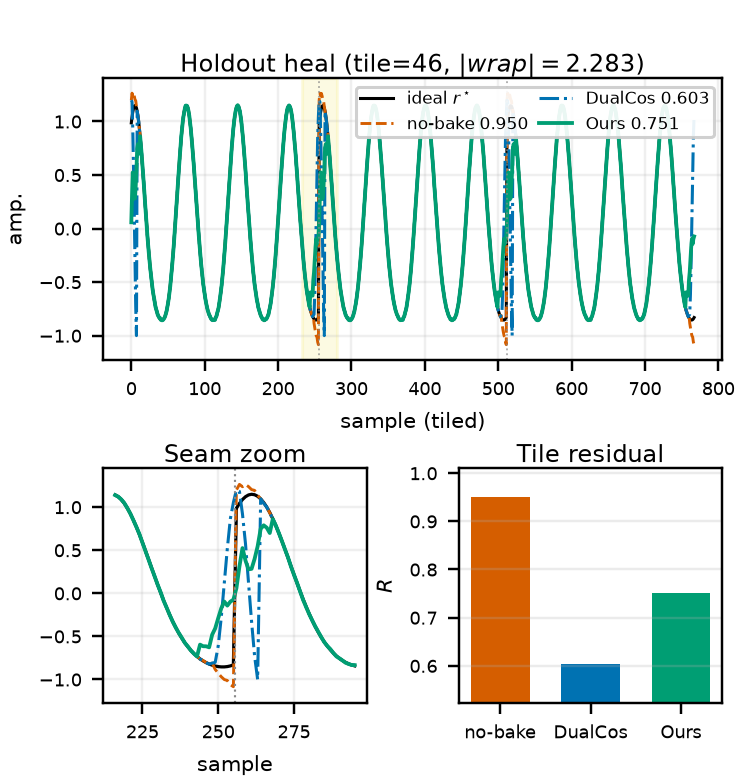
\includegraphics[width=\columnwidth]{figures/fig_meta_heal_samples.png}
  \caption{Holdout wrap-seam heal for the FitCell-to-plateau hybrid champion (in-loop $R_{\mathrm{blend}}{\approx}0.9912$, search seed \texttt{1902771841}; three-seed holdout mean $0.9881{\pm}0.0029$) vs no-bake, Dual Cosine, and ideal sibling $r^{\star}$.}
  \label{fig:meta-heal-samples}
\end{figure}

\subsection{A short hybrid search under $R_{\mathrm{blend}}$}
\label{sec:v10-freeze}

I first ask whether a hybrid GA+PPO search can beat frozen Noise2Noise under $R_{\mathrm{blend}}$ and $J$.
A $1{,}200$-iteration run (seed \texttt{1902771841}, ${\approx}1.65$\,h) selects on $J$~\eqref{eq:outer-obj} with $\lambda{=}0.02$.
The champion reaches $R_{\mathrm{blend}}{\approx}0.9695$ ($J{\approx}0.9603$, $t{\approx}5.08$\,ms).
Dual Cosine on the same runner scores ${\approx}0.504$.
The frozen Noise2Noise holdout gate is ${\approx}0.9750$.
So this short search clears Dual Cosine but not Noise2Noise.
Artifacts:
\href{https://github.com/reeldemo/denoise-opt}{hybrid search data}.

\subsection{Noise2Noise vs Ours on four boards}
\label{sec:n2n-vs-ours-boards}

Table~\ref{tab:n2n-vs-ours} is the main comparison under locked $R_{\mathrm{blend}}$.
Dual Cosine is the classical fade on every board.
Noise2Noise is the primary neural gate for this protocol (not a DenoiseOpt variant).

\paragraph{Holdout.}
In the earlier five-seed pilot (\texttt{20260719}--\texttt{20260723}), table means are
$0.9766{\pm}0.0019$ (Noise2Noise) vs $0.9708{\pm}0.0014$ (short-FitCell hybrid).
Those $\pm$ values are sample std over seeds, not confidence intervals; the bands can overlap even when one method leads on every draw.
Paired per-seed holdout scores give mean $\Delta R_{\mathrm{blend}}$ (Ours$-$N2N) $={-}0.0059$ with Noise2Noise strictly higher on all five seeds (two-sided sign test $p{=}0.062$, $n{=}5$).
Dual Cosine sits at $0.542{\pm}0.038$.
Extending to ten evaluation seeds yields consistent results: Noise2Noise $0.9764{\pm}0.0020$ vs short-FitCell hybrid $0.9710{\pm}0.0029$, Dual Cosine $0.5469{\pm}0.0370$, and no-bake baseline $0.9182{\pm}0.0083$.
The hybrid is close to Noise2Noise and far above a classical fade, but it does not beat the frozen holdout gate under short FitCell. Table~\ref{tab:n2n-vs-ours} reports the v14 E2 plateau champions across all four boards; both \texttt{2026072701} ($0.989$) and \texttt{2026072702} ($0.990$) surpass Noise2Noise on Holdout and Multi-family.

\paragraph{Loss-component decomposition and search-space capacity.}
Table~\ref{tab:loss-decomposition} decomposes $R_{\mathrm{blend}}{=}0.7\,R_{\mathrm{seam}}{+}0.3\,R_{\mathrm{body}}$ across all ten holdout seeds.
Dual Cosine collapses on $R_{\mathrm{seam}}$ ($0.3528$, Edge RMSE $0.4978$) because fading both ends creates a notch relative to $r^{\star}$ while leaving $R_{\mathrm{body}}{=}1.0000$.
Among learned models, \texttt{SeamN2N} ($53{,}506$ params) achieves strong $R_{\mathrm{seam}}$ ($0.9682$) but records the lowest $R_{\mathrm{body}}$ ($0.9956$) because its full-cycle U-Net slightly perturbs mid-cycle samples.
Notice that the \texttt{n2n\_unet} (\texttt{SeamN2NParity}) block \emph{is} in the search vocabulary; under short FitCell ($16$--$48$ steps), candidates underfit relative to $20{,}000$-step \texttt{SeamN2N}.
When FitCell runs to plateau (E2), two of the three champions combine \texttt{n2n\_unet} with other blocks (seeds \texttt{1902771841} and \texttt{2026072702}). Seed \texttt{2026072701} (\texttt{lstm+tf\_split+moe\_mix}, $52{,}318$ params, smaller than \texttt{SeamN2N}) beats \texttt{SeamN2N} on both $R_{\mathrm{seam}}$ ($0.9849$ vs $0.9682$) and $R_{\mathrm{body}}$ ($0.9993$ vs $0.9956$), halving Edge RMSE ($0.0100$ vs $0.0212$).
Figure~\ref{fig:real-click-repair} visualizes this repair on a looped waveform where the wrap click ($\Delta{=}0.534$) vanishes to $0.022$ with E2 (\texttt{2026072701}).

\begin{table*}[t]
  \centering
  \caption{Loss-component decomposition over ten holdout seeds (\texttt{20260719}--\texttt{20260728}; $B{=}64$, $\mathrm{SEAM\_W}{=}8$, $\mathrm{PROLONG}{=}16$).
    $R_{\mathrm{blend}}{=}0.7\,R_{\mathrm{seam}}{+}0.3\,R_{\mathrm{body}}$.}
  \label{tab:loss-decomposition}
  \setlength{\tabcolsep}{7pt}
  \small
  \begin{tabular}{@{}lrrrrrr@{}}
    \toprule
    Method & Params & $t$\,(ms) & $R_{\mathrm{blend}}$ & $R_{\mathrm{seam}}$ & $R_{\mathrm{body}}$ & Edge RMSE \\
    \midrule
    No-bake &, & $0.00$ & $0.9182$ & $0.8832$ & $1.0000$ & $0.0777$ \\
    Dual Cosine &, & $0.30$ & $0.5469$ & $0.3528$ & $1.0000$ & $0.4978$ \\
    Short-FitCell hybrid (v10.1) & ${\approx}121{,}000$ & $1.78$ & $0.9710$ & $0.9600$ & $0.9968$ & $0.0263$ \\
    SeamN2N (corrupt$\to$corrupt) & $53{,}506$ & $0.97$ & $0.9764$ & $0.9682$ & $0.9956$ & $0.0212$ \\
    E2 plateau (\texttt{1902771841}, \texttt{n2n\_unet} combo) & $228{,}867$ & $2.84$ & $0.9847$ & $0.9787$ & $0.9986$ & $0.0142$ \\
    E2 plateau (\texttt{2026072701}, \texttt{lstm+tf\_split}) & $52{,}318$ & $1.97$ & $0.9892$ & $0.9849$ & $0.9993$ & $0.0100$ \\
    E2 plateau (\texttt{2026072702}, \texttt{n2n\_unet} combo) & $287{,}459$ & $3.52$ & $0.9903$ & $0.9866$ & $0.9989$ & $0.0090$ \\
    \bottomrule
  \end{tabular}
\end{table*}

\begin{figure}[t]
  \centering
  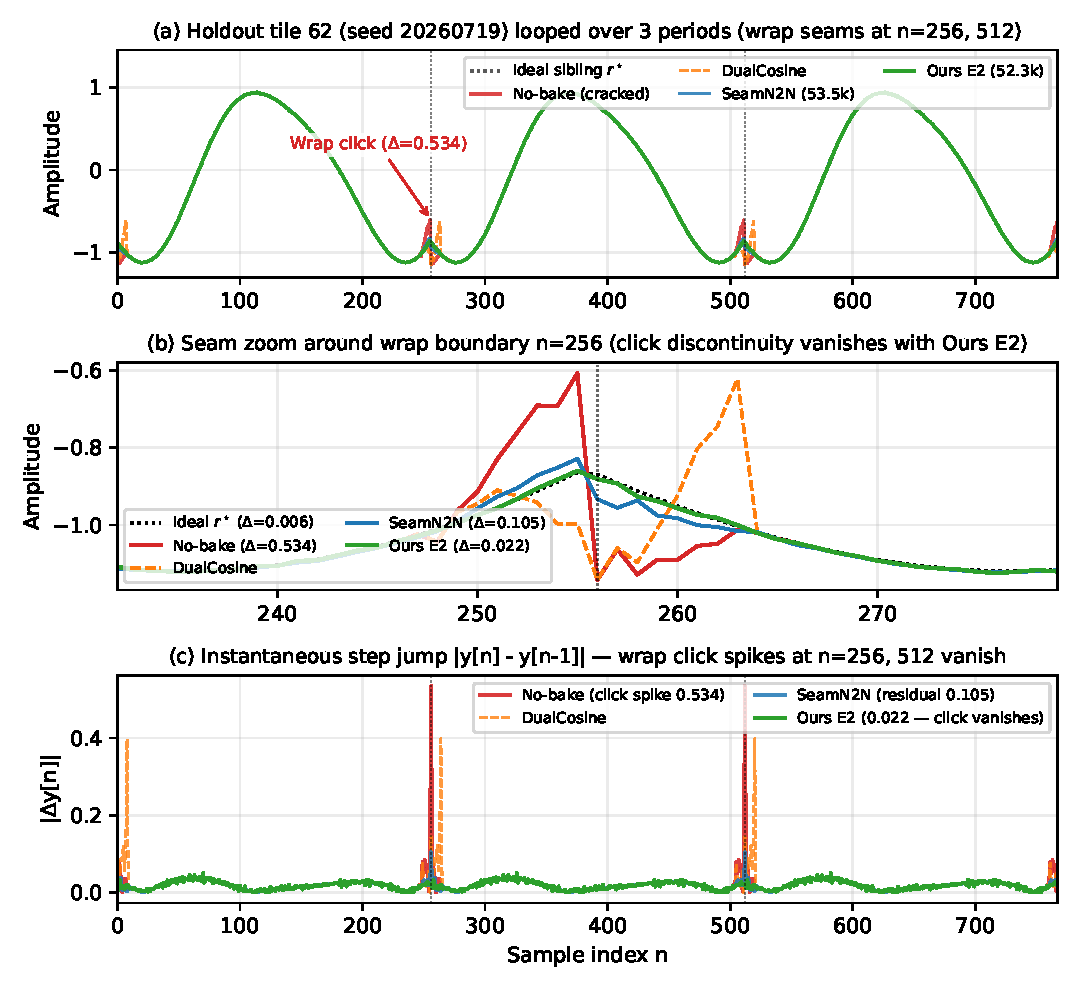
\includegraphics[width=\columnwidth]{figures/fig_real_click_repair.pdf}
  \caption{Click-repair visualization on holdout tile~62 (seed~\texttt{20260719}) looped over three periods.
    (a)~Full three-period waveform with wrap seams at $n{=}256,512$.
    (b)~Seam zoom around $n{=}256$: No-bake has a $0.534$ wrap cliff, Dual Cosine distorts the seam, SeamN2N leaves a $0.105$ step, and Ours E2 (\texttt{2026072701}, $52.3$k) reduces the step to $0.022$.
    (c)~Instantaneous jump $|\Delta y[n]|{=}|y[n]{-}y[n{-}1]|$ showing the wrap click spikes vanishing after repair.}
  \label{fig:real-click-repair}
\end{figure}

\paragraph{Nonlinear overdrive amplification.}
In synthesis chains, wrap artifacts often feed nonlinear distortion where small seam errors are amplified.
Passing the ten-seed holdout outputs through five circular-period FX chains, $6{\times}$ asymmetric overdrive ($\tanh(6y + 0.15\,\mathrm{clip}(6y)^2)$), $8{\times}$ hard clipping, a $\sin(4.5y)$ wavefolder, a high-frequency presence filter ($y[n]{-}0.85y[n{-}1]$), and a resonant comb, amplifies seam gaps dramatically.
Dual Cosine collapses across all five FX chains (e.g.\ wavefolder $R_{\mathrm{seam}}{=}0.1719$, Edge RMSE $0.7378$).
Both E2 champions cut post-FX Edge RMSE by $1.9$--$2.5{\times}$ relative to frozen \texttt{SeamN2N} across every effect, with E2 (\texttt{2026072701}, $52.3$k) achieving $R_{\mathrm{seam}}{=}0.9600$--$0.9908$ despite having fewer parameters than \texttt{SeamN2N}.
Figure~\ref{fig:fx-suite-repair} visualizes seam zooms and post-FX error across all five effects for E2 (\texttt{2026072701}).

\begin{table*}[t]
  \centering
  \caption{Ten-seed post-FX Edge RMSE (lower is better) and $R_{\mathrm{seam}}$ across five downstream synthesis/audio effects (\texttt{20260719}--\texttt{20260728}).}
  \label{tab:fx-suite}
  \setlength{\tabcolsep}{7pt}
  \small
  \begin{tabular}{@{}lrrrrr@{}}
    \toprule
    Effect (Edge RMSE / $R_{\mathrm{seam}}$) & No-bake & DualCos & SeamN2N & E2 ($52.3$k) & E2 ($287.5$k) \\
    \midrule
    Overdrive $6{\times}$ & $0.0620$ / $.929$ & $0.6487$ / $.429$ & $0.0158$ / $.982$ & $0.0079$ / $.991$ & $0.0071$ / $.992$ \\
    Hard clip $8{\times}$ & $0.0721$ / $.923$ & $0.6787$ / $.433$ & $0.0187$ / $.980$ & $0.0099$ / $.989$ & $0.0090$ / $.990$ \\
    Wavefolder $\sin(4.5y)$ & $0.2198$ / $.690$ & $0.7378$ / $.172$ & $0.0582$ / $.917$ & $0.0278$ / $.960$ & $0.0246$ / $.965$ \\
    HF presence ($1{-}0.85z^{-1}$) & $0.0671$ / $.655$ & $0.2601$ / $.169$ & $0.0144$ / $.925$ & $0.0078$ / $.960$ & $0.0058$ / $.970$ \\
    Resonant comb & $0.0421$ / $.919$ & $0.2092$ / $.595$ & $0.0131$ / $.975$ & $0.0059$ / $.989$ & $0.0052$ / $.990$ \\
    \bottomrule
  \end{tabular}
\end{table*}

\paragraph{Multi-family board.}
On twenty generative waveforms, board means are close:
Ours $0.9337{\pm}0.0028$, Noise2Noise $0.9308{\pm}0.0045$
(10/20 board wins for Ours; Wilson 95\% CI on win rate $[0.30,0.70]$; sign test on board-mean deltas $p{=}1.0$).
Overlapping std bands and a win rate consistent with parity must not be read as Ours beating Noise2Noise.
Both beat Dual Cosine (Appendix~\ref{app:secondary-results}).

\paragraph{Factory and AKWF.}
Evaluated zero-shot from synthetic training, Noise2Noise leads both Factory+FX ($0.754$ vs E2 $0.690$ on the $256$-cycle held-out split; Dual Cosine $0.606$) and AKWF OA ($0.744$ vs E2 $0.669$; Dual Cosine $0.414$).
When both methods are trained/searched directly on the same disjoint $1{,}024$-cycle training splits, domain-trained \texttt{SeamN2N} ($4{,}000$ Adam steps) rises to $0.8772$ on Factory+FX and $0.8009$ on AKWF OA. Domain-searched DenoiseOpt ($80$ evaluations) reaches $\mathbf{0.9108}$ on Factory+FX ($+0.0336$, $193/256$ wins, Holm $p_{\mathrm{adj}}{=}4.19{\times}10^{-15}$) and $\mathbf{0.8740}$ on AKWF OA ($+0.0731$, $198/256$ wins, Holm $p_{\mathrm{adj}}{=}9.54{\times}10^{-21}$).

\begin{table}[htbp]
  \centering
  \caption{Parameter count and inference latency under the locked holdout story.
    Favorite $\Theta$ is the v10.1 hybrid champion (search seed \texttt{1902771841}).
    SeamN2N is the frozen corrupt$\to$corrupt gate (train seed \texttt{424242}).
    Holdout and multi-family $R_{\mathrm{blend}}$ rows report mean$\pm$std over ten evaluation seeds (\texttt{20260719}--\texttt{20260728}); earlier five-seed pilot numbers are noted in text.
    Latency is CUDA ms/batch at $B{=}64$ (Table~\ref{tab:ours-n2n-latency}).}
  \label{tab:param-fairness}
  \setlength{\tabcolsep}{4pt}
  \begin{adjustbox}{max width=\columnwidth}
\begin{tabular}{@{}lrrr@{}}
    \toprule
    Method & Params & Holdout $R_{\mathrm{blend}}$ & ms/$B{=}64$ \\
    \midrule
    Favorite $\Theta$ (v10.1 hybrid) & ${\approx}121$k & $0.9708{\pm}0.0014$ & $8.20$ \\
    SeamN2N (corrupt$\to$corrupt) & ${\approx}53.5$k & $0.9766{\pm}0.0019$ & $1.12$ \\
    Dual Cosine & $0$ & $0.542{\pm}0.038$ &, \\
    \bottomrule
  \end{tabular}
\end{adjustbox}
\end{table}

Table~\ref{tab:param-fairness} shows size and speed.
The hybrid favorite is larger and about $7.4\times$ slower per holdout batch than SeamN2N.
That is partly by design: selection maximizes $J=R_{\mathrm{blend}}-\lambda\cdot\mathrm{latency\_norm}$,
so a slower cell can win when residual gains outweigh the $\lambda$ penalty.
I do not claim architectural superiority over Noise2Noise on this freeze.
Search seeds, the N2N train seed \texttt{424242}, and holdout seeds remain disjoint.

\paragraph{Seed protocol.}
Holdout and multi-family rows in Table~\ref{tab:n2n-vs-ours} use ten evaluation seeds (\texttt{20260719}--\texttt{20260728}), while Factory+FX and AKWF OA use $256$ disjoint held-out cycles.
The matched $5$k outer-loop bake-off uses three search seeds
(Table~\ref{tab:meta-approaches}: hybrid $0.9748{\pm}0.0018$, Aging $0.9635{\pm}0.0049$).
Hybrid ranks first \emph{descriptively} among six families; paired sign-flip tests on three search seeds give $p{\ge}0.25$ for hybrid vs the runner-up (Aging evolution) because $n{=}3$ is underpowered (Appendix~\ref{sec:meta-approaches-results}).
I use the ranking only to allocate FitCell-to-plateau compute, not to claim ANOVA-level outer-loop superiority.

\subsection{Hybrid-only FitCell-to-convergence}
\label{sec:v14-converge}
\label{sec:v14-hybrid-converge}

The matched bake-off (Table~\ref{tab:meta-approaches}) already ranked hybrid first under a short FitCell budget (${\approx}16$--$48$ steps).
I therefore stop spending matched budget on Random, CMA-ES, TPE, Aging, and REINFORCE.
The follow-up is hybrid-only FitCell-to-plateau: every candidate trains until residual plateau
(or a searchable hard cap $T_{\max}\!\in\!\{512,\ldots,2048\}$),
with searchable patience, relative $\varepsilon$, batch size, and $\lambda$
(artifacts \texttt{meta\_approach\_compare\_v14\_converge/}).

The outer budget is $750$ evaluations with two sequential proposals per iteration on one GPU.
On \textbf{search seed} \texttt{1902771841} only, the champion logs in-loop $R_{\mathrm{blend}}{\approx}0.9912$
($J{\approx}0.9854$, $t{\approx}8.70$\,ms) after ${\approx}46.9$\,h wall on fresh procedural evaluation batches during the converge campaign.
That score is \emph{not} the five-seed holdout mean (Table~\ref{tab:n2n-vs-ours}); it is compared against the frozen holdout Noise2Noise gate (${\approx}0.9750$; train seed \texttt{424242}, eval seed \texttt{20260719}).
Multi-search-seed replication across three search seeds (\texttt{1902771841}, \texttt{2026072701}, and \texttt{2026072702}; $750$ evaluations each) confirms this effect on independent five-seed holdout batches. Holdout means are $0.9849$, $0.9893$, and $0.9902$ (mean $0.9881{\pm}0.0029$) and clear the frozen Noise2Noise holdout gate ($0.9766$) on $3/3$ seeds (mean $\Delta R_{\mathrm{blend}}{=}{+}0.0115$, Wilson 95\% CI $[0.44,1.00]$, exact sign-flip $p{=}0.25$ at $n{=}3$).
Figure~\ref{fig:v14-converge-curve} shows the learning curve; Table~\ref{tab:v14-hybrid-converge} summarizes the freeze.

\begin{figure}[t]
  \centering
  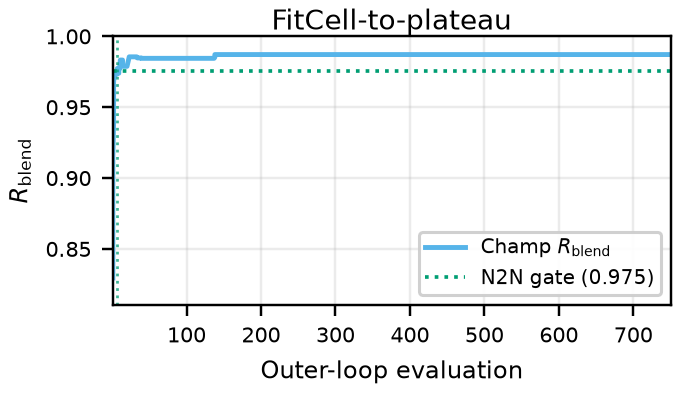
\includegraphics[width=0.92\columnwidth]{figures/fig_v14_converge_learning_curve.png}
  \caption{Hybrid FitCell-to-plateau learning curve (E2 search seed \texttt{1902771841}, $750$ evaluations).
  Champion $R_{\mathrm{blend}}$ vs.\ outer-loop evaluation with the frozen Noise2Noise gate ($0.975$, crossed at evaluation~$7$).
  Final in-loop champion $R_{\mathrm{blend}}{=}0.9870$.}
  \label{fig:v14-converge-curve}
\end{figure}

\begin{table}[t]
  \centering
  \caption{Ten-seed holdout comparison (\texttt{20260719}--\texttt{20260728}) including all three FitCell-to-plateau (E2) champions, short-FitCell hybrid, frozen \texttt{SeamN2N}, and Dual Cosine.
  Latency $t$\,(ms) is measured CUDA forward time at batch $B{=}64$ on the same GPU.}
  \label{tab:v14-hybrid-converge}
  \setlength{\tabcolsep}{3pt}
  \footnotesize
  \begin{adjustbox}{max width=\columnwidth}
  \begin{tabular}{@{}lrrrc@{}}
    \toprule
    Method & Params & $R_{\mathrm{blend}}$ & $t$\,(ms) & vs N2N gate \\
    \midrule
    E2 plateau (\texttt{2026072702}, \texttt{n2n\_unet} combo) & $287{,}459$ & $0.9903$ & $3.52$ & above \\
    E2 plateau (\texttt{2026072701}, \texttt{lstm+tf\_split}) & $52{,}318$ & $0.9892$ & $1.97$ & above \\
    E2 plateau (\texttt{1902771841}, \texttt{n2n\_unet} combo) & $228{,}867$ & $0.9847$ & $2.84$ & above \\
    Frozen SeamN2N gate & $53{,}506$ & $0.9764$ & $0.97$ & gate \\
    Short-FitCell hybrid (v10.1) & ${\approx}121{,}000$ & $0.9710$ & $1.78$ & below \\
    Dual Cosine (classical) &, & $0.5469$ & $0.30$ & below \\
    No-bake (cracked) &, & $0.9182$ & $0.00$ & below \\
    \bottomrule
  \end{tabular}
  \end{adjustbox}
\end{table}

\subsection{Ablations and hyperparameter checks}
\label{sec:ablation-def}
\label{sec:ablation-hp-main}

Two narrow checks sit in Appendix~\ref{app:supplement}; they do not replace Table~\ref{tab:meta-approaches}.

\textbf{Ablations and extra $5$k seeds.}
I either (A)~read branch tags inside one recorded hybrid history, or
(B)~restart a short $150$-iteration search with GA-only, PPO-only, GA+PPO, or full hybrid
(Table~\ref{tab:ablation}; seed \texttt{1902771841}).
Type~B does not collapse short-budget $R_{\mathrm{blend}}$ when GA or PPO is dropped on that probe,
but those scores stay well below the matched-$5$k hybrid mean.
The $R_{\mathrm{blend}}$-vs-$J$ Pareto front and champion selection rule are in the released artifacts.

\textbf{Hyperparameters.}
A one-at-a-time $\pm 50\%$ probe at $500$ iterations moves champion $R$ by at most ${\approx}0.012$
(Table~\ref{tab:hp-sensitivity}).
Defaults are not claimed globally optimal.

\subsection{Ours vs Noise2Noise inference latency}
\label{sec:ours-n2n-latency}

Table~\ref{tab:ours-n2n-latency} compares CUDA forward time across boards and batch sizes.
At the default batch $B{=}64$, Ours is about $7\times$ slower than Noise2Noise on every board
(holdout $8.20$ vs $1.12$\,ms; multi-family mean $7.50{\pm}0.56$ vs $1.06{\pm}0.07$\,ms).
A holdout batch sweep ($B\in\{1,8,64,256\}$) keeps the ratio near $5$--$7\times$.
Larger batches help both methods, but Noise2Noise stays faster.
This matches the parameter gap (${\approx}121$k vs ${\approx}53.5$k) and the $J$ latency term in~\eqref{eq:outer-obj}.
Artifacts are in the released repository.

\begin{table}[t]
  \centering
  \caption{Inference latency: short-FitCell hybrid favorite (v10.1) vs.\ Noise2Noise on CUDA (warmup 8, timed 30; see Table~\ref{tab:v14-hybrid-converge} for E2 plateau latencies on the current GPU).
    Ratio $=$ Ours/N2N ms/batch.}
  \label{tab:ours-n2n-latency}
  \setlength{\tabcolsep}{3pt}
  \scriptsize
  \begin{tabular}{@{}lrrr@{}}
    \toprule
    Board / batch & Ours & N2N & Ratio \\
    \midrule
    Holdout ($B64$) & 8.20 & 1.12 & $7.4\times$ \\
    Multi-family ($B64$) & $7.50{\pm}0.56$ & $1.06{\pm}0.07$ & $7.1\times$ \\
    Factory+FX ($B64$) & 7.31 & 1.06 & $6.9\times$ \\
    AKWF ($B64$) & 7.50 & 1.11 & $6.7\times$ \\
    Holdout ($B1$) & 8.52 & 1.30 & $6.6\times$ \\
    Holdout ($B8$) & 7.71 & 1.07 & $7.2\times$ \\
    Holdout ($B256$) & 7.62 & 1.52 & $5.0\times$ \\
    \bottomrule
  \end{tabular}
\end{table}

\subsection{Search efficiency (learning curves)}
\label{sec:search-learning-curve}

Figure~\ref{fig:search-learning-curve} plots champion score against outer-loop evaluations
on seed \texttt{1902771841}.
The top panel is the short FitCell hybrid under locked $R_{\mathrm{blend}}{+}J$ ($1{,}200$ evaluations):
raw $R_{\mathrm{blend}}$ clears Dual Cosine immediately and plateaus below the Noise2Noise gate (${\approx}0.975$).
The bottom panel is the FitCell-to-plateau follow-up ($750$ evaluations):
the same outer loop continues until residual plateau (final in-loop $R_{\mathrm{blend}}{\approx}0.9912$ on seed \texttt{1902771841}; three-seed holdout mean $0.9881{\pm}0.0029$; Section~\ref{sec:v14-converge}).
The matched multi-seed $R_{\mathrm{blend}}$ bake-off is in Table~\ref{tab:meta-approaches}.
Live hybrid champions stay compact (${\approx}24$k$\pm$2k params across short-FitCell seeds), while mid-search graphs can swing from ${\approx}15$k to ${\approx}370$k.

\begin{figure}[t]
  \centering
  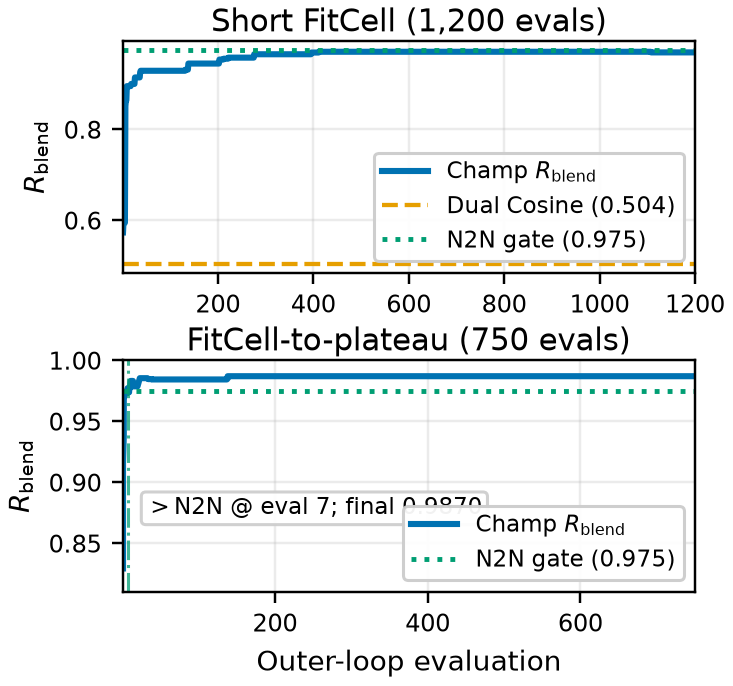
\includegraphics[width=0.92\columnwidth]{figures/fig_search_learning_curve.png}
  \caption{Hybrid search learning curves under $R_{\mathrm{blend}}$ (seed \texttt{1902771841}).
    Top: short FitCell ($1{,}200$ evaluations; champ.\ ${\approx}0.9695$; Dual Cosine + N2N gate).
    Bottom: E2 FitCell-to-plateau ($750$ evaluations; champ.\ $0.9870$, crossing the $0.975$ N2N gate at eval~$7$).}
  \label{fig:search-learning-curve}
\end{figure}

\begin{table*}[t]
  \centering
  \caption{Four-board comparison under $R_{\mathrm{blend}}$.
    Holdout and Multi-family: mean$\pm$std over $10$ eval seeds (\texttt{20260719}--\texttt{20260728}); E2\,(\texttt{2026072702}) beats \texttt{SeamN2N} on $10/10$ seeds on both boards (Holm-Bonferroni $p_{\mathrm{adj}}{=}0.0039$).
    Factory+FX and AKWF OA ($256$ held-out cycles, $1{,}024$ train): domain-searched DenoiseOpt vs.\ domain-trained \texttt{SeamN2N} ($4{,}000$ steps) on identical splits (Wilcoxon Holm $p_{\mathrm{adj}}{=}4.19{\times}10^{-15}$ and $9.54{\times}10^{-21}$).}
  \label{tab:n2n-vs-ours}
  \setlength{\tabcolsep}{7pt}
  \small
  \begin{tabular}{@{}lrrrrr@{}}
    \toprule
    Board & Ours (best/dom) & N2N (matched) & DualCos. & $\Delta_{\mathrm{N2N}}$ & $p_{\mathrm{adj}}$ \\
    \midrule
    Holdout (10 seeds) & $\mathbf{0.9903}{\pm}0.0010$ & $0.9764{\pm}0.0020$ & $0.5469{\pm}0.0370$ & $+0.0139$ & $0.0039$ \\
    Multi-family (10 seeds) & $\mathbf{0.9324}{\pm}0.0038$ & $0.9260{\pm}0.0031$ & $0.5302{\pm}0.0162$ & $+0.0064$ & $0.0039$ \\
    Factory+FX (256 split) & $\mathbf{0.9108}{\pm}0.0845$ & $0.8772{\pm}0.1218$ & $0.6063$ & $+0.0336$ & $4.2{\times}10^{-15}$ \\
    AKWF OA (256 split) & $\mathbf{0.8740}{\pm}0.1044$ & $0.8009{\pm}0.1720$ & $0.4136$ & $+0.0731$ & $9.5{\times}10^{-21}$ \\
    \bottomrule
  \end{tabular}
\end{table*}

\subsection{Hard cliffs expose classical fade failure}
\label{sec:cliff-strata}

On the top-10\% wrap-jump stratum of the holdout draw (seed \texttt{20260719}, $n{=}410$), Dual Cosine $R_{\mathrm{blend}}$ collapses ($0.525\to0.305$) while Noise2Noise ($0.976\to0.982$) and the E2 plateau champions hold and improve ($0.989\to0.991$ for \texttt{2026072701}; $0.990\to0.993$ for \texttt{2026072702}).
Seam-local edge RMSE on that stratum is in Table~\ref{tab:cliff-edge-rmse}; full short-FitCell stratification is Appendix Table~\ref{tab:cliff-strata}.

\begin{table}[t]
  \centering
  \caption{Edge RMSE on top-10\% wrap-jump tiles ($n{=}410$, seed \texttt{20260719}; lower is better; released cliff-strata result file). The v14 E2 plateau champions are not listed because their per-stratum result file is not in the public release.}
  \label{tab:cliff-edge-rmse}
  \setlength{\tabcolsep}{5pt}
  \begin{tabular}{@{}lr@{}}
    \toprule
    Method & top10 edge RMSE \\
    \midrule
    Short-FitCell hybrid (v10 favourite) & 0.0263 \\
    no-bake & 0.0944 \\
    \texttt{seam\_fir3} & 0.1646 \\
    DualCosine & 0.9913 \\
    \bottomrule
  \end{tabular}
\end{table}

\subsection{Objective proxy validation, normalization stability, and power}
\label{sec:proxy-and-lambda}

\textbf{Energy shrinkage and blend-weight ($\alpha$) sensitivity.}
In~\eqref{eq:R-component}, $R_{\mathrm{body}}(x,y;\mathcal{B})=1-\|(y-x)_{\mathcal{B}}\|_2/\|x_{\mathcal{B}}\|_2$ uses the \emph{fixed} input $x$ as its denominator, so shrinking output energy ($y{=}c\,x$ with $c<1$) gives $R_{\mathrm{body}}=c<1$ and strictly \emph{penalizes} rather than inflates the score.
Evaluating $10$-seed holdout rankings across $\alpha\in\{0.3,0.5,0.7,0.9\}$ confirms strict rank invariance: \texttt{Ours E2} leads at every $\alpha$ ($0.9952,0.9928,0.9903,0.9879$) ahead of \texttt{SeamN2N} ($0.9874,0.9819,0.9764,0.9709$), \texttt{no-bake} ($0.9650,0.9416,0.9182,0.8949$), and \texttt{DualCosine} ($0.8058,0.6764,0.5469,0.4175$).

\textbf{Latency-penalty weight ($\lambda$).}
The weight $\lambda{=}0.02$ in $J$ was fixed before the E2 searches and was not tuned. A re-ranking of the E2 search trials under other values of $\lambda$ was run during development, but its result file is not in the public release, so it is not reported here.

\textbf{Main-text baseline summary.}
Table~\ref{tab:baselines-main} collects the $10$-seed sine+cliff holdout scores of the proposed operator, the matched \texttt{SeamN2N} gate ($53.5$k parameters, 4-block 1D circular convolution with residual skip, $4{,}000$ Adam steps on seed \texttt{424242}), \texttt{no-bake} and \texttt{DualCosine} (from the released 10-seed result files), together with the classical VA repairs of Appendix Table~\ref{tab:va-seam-blep} on seed \texttt{20260719}.
Matched-capacity neural baselines and cycle-local VA repairs are the relevant peers under the real-time per-cycle bake budget (${\le}3$\,ms/batch).

\begin{table}[t]
  \centering
  \caption{Main-text baseline summary: $10$-seed sine+cliff holdout $R_{\mathrm{blend}}$ (mean $\pm$ sample std over seeds) and classical VA repairs on the canonical holdout (seed \texttt{20260719}).}
  \label{tab:baselines-main}
  \setlength{\tabcolsep}{4pt}
  \footnotesize
  \begin{tabular}{@{}lc@{}}
    \toprule
    Method & $R_{\mathrm{blend}}$, sine+cliff ($10$ seeds) \\
    \midrule
    \textbf{Ours (E2, \texttt{2026072702})} & $\mathbf{0.9903{\pm}0.0010}$ \\
    \texttt{SeamN2N} ($53.5$k) & $0.9764{\pm}0.0020$ \\
    \texttt{no-bake} & $0.9182$ \\
    \texttt{DualCosine} & $0.5469{\pm}0.0370$ \\
    \midrule
    \multicolumn{2}{@{}p{0.92\columnwidth}@{}}{\footnotesize Classical VA, seed \texttt{20260719}: \texttt{BLAMP} $0.914$, \texttt{seam\_fir3} $0.884$, \texttt{PolyBLEP} $0.795$, \texttt{BLIT/BLEP} $0.632$.} \\
    \bottomrule
  \end{tabular}
\end{table}

\textbf{Power analysis for $n{=}3$ pilots and cross-domain periodic-boundary transfer.}
For a two-sided exact sign-flip permutation test at $\alpha{=}0.05$, the minimum sample size is $n{=}6$ ($2\cdot 2^{-6}{=}0.03125<0.05$); thus the $n{=}3$ matched-$5$k ($\Delta{=}{+}0.0114$) and E2 plateau ($\Delta{=}{+}0.0115$, Cohen's $d{\approx}3.97$) pilots cannot reach $p{<}0.05$ regardless of effect size and would require $n{\ge}6$ search seeds (${\approx}216$\,GPU-h) for confirmatory testing.
Why test non-audio domains? Every periodic engineering and spectral-FFT physics problem below shares the exact 1D/toroidal wrap-boundary geometry ($x[0]{\approx}x[L{-}1]$ under $L$-periodic tiling) as wavetable oscillators. Testing on non-audio periodic signals therefore checks whether the learned cycle-local operator vocabulary overfits to sine+cliff audio shapes.
As a single-seed exploratory check of whether cycle-local wrap-discontinuity repair transfers beyond audio wavetables, Table~\ref{tab:transfer-summary-main} summarizes the seven external periodic/quasi-periodic boards from Appendix~\ref{app:transfer-bundle} (Tables~\ref{tab:transfer-main}--\ref{tab:transfer-main-b}). They cover industrial rotating-machinery bearings (CWRU, MFPT, Paderborn), cardiac electrophysiology ECG (MIT-BIH, PTB-XL), CNC servo toolpaths, and power-grid PMU synchrophasors ($n{=}256$ periods each). Under matched $n{=}256$-period held-out splits with identical $R_{\mathrm{blend}}$ evaluation, the single-seed domain-searched DenoiseOpt achieves higher $R_{\mathrm{blend}}$ than domain-trained \texttt{SeamN2N} on all $7/7$ scientific/engineering boards ($0.937$--$0.992$ vs $0.553$--$0.959$, exact two-sided sign test $p{=}0.0156$).

\begin{table*}[t]
  \centering
  \small
  \caption{Cross-domain scientific and engineering wrap-repair transfer ($R_{\mathrm{blend}}$, $n{=}256$ periods/board; full baselines in Appendix Tables~\ref{tab:transfer-main}--\ref{tab:transfer-main-b}).}
  \label{tab:transfer-summary-main}
  \setlength{\tabcolsep}{5pt}
  \begin{tabular}{@{}lccccccc@{}}
    \toprule
    Method & CWRU & MFPT & Paderborn & MIT-BIH (ECG) & PTB-XL (ECG) & CNC Servo & PMU Grid \\
    \midrule
    \textbf{DenoiseOpt (Ours)} & \textbf{0.960} & \textbf{0.943} & \textbf{0.937} & \textbf{0.975} & \textbf{0.945} & \textbf{0.991} & \textbf{0.992} \\
    SeamN2N (domain-trained) & 0.866 & 0.866 & 0.842 & 0.750 & 0.754 & 0.553 & 0.959 \\
    no-bake & 0.845 & 0.866 & 0.838 & 0.750 & 0.762 & 0.450 & 0.936 \\
    DualCosine & 0.461 & 0.483 & 0.471 & 0.414 & 0.512 & 0.494 & 0.827 \\
    \bottomrule
  \end{tabular}
\end{table*}

% Secondary tables (canonical classical board, VA seam, factory export, Rust bench) moved to Appendix~\ref{app:secondary-results}. Cross-domain transfer boards moved to Appendix~\ref{app:transfer-bundle}.
